\section{Results}
\label{sec:results}

\subsection{Delaunay triangulation algorithm}
\label{sub:results:triangulation}

We tested the Bowyer-Watson and Lawson triangulation algorithms for randomly generated inputs of different size.
%This is done by recursively adding $n$ points to the initial triangulation.

For each input size, 40 trials were performed.
In Figure \ref{fig:triangulation-runtime} we can see the average time that was needed for inserting the points.
We see that both algorithms don't differ much from each other, but Lawson's triangulation method seems slighty faster than Bowyer-Watsons.

%The result without PSLG boundary segments is shown in Figure \ref{fig:triangulation/runtime} and
%with the segments in Figure \ref{fig:result_runtimeSegments}.

We repeated the same experiments for a constrained triangulation problem.
In addition to the random generated vertices, we now added a PSLG that contrained the way in way the triangulation is performed.
The results are in Figure \ref{fig:triangulation-pslg-runtime}.
Again the difference between the methods is fairly small.

\begin{figure}[ht]
    \centering
    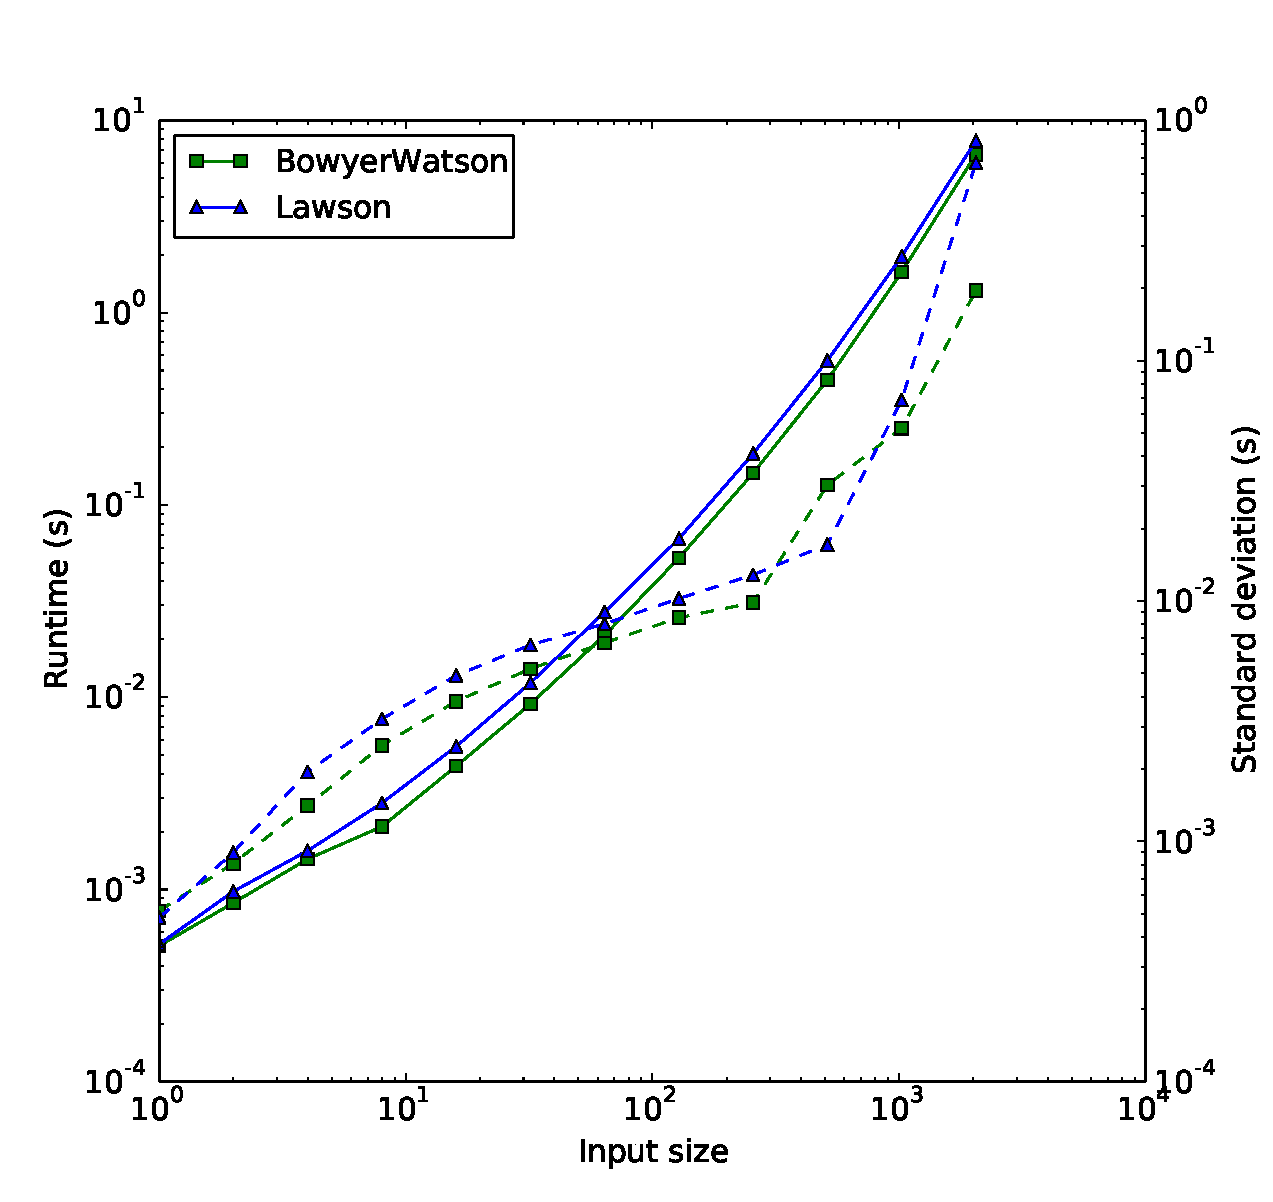
\includegraphics[width=\columnwidth]{../images/runtime.pdf}
    \label{fig:triangulation-runtime}
    \caption{Runtime for triangulation algorithms when input is unconstrained}
\end{figure}

\begin{figure}[ht]
    \centering
    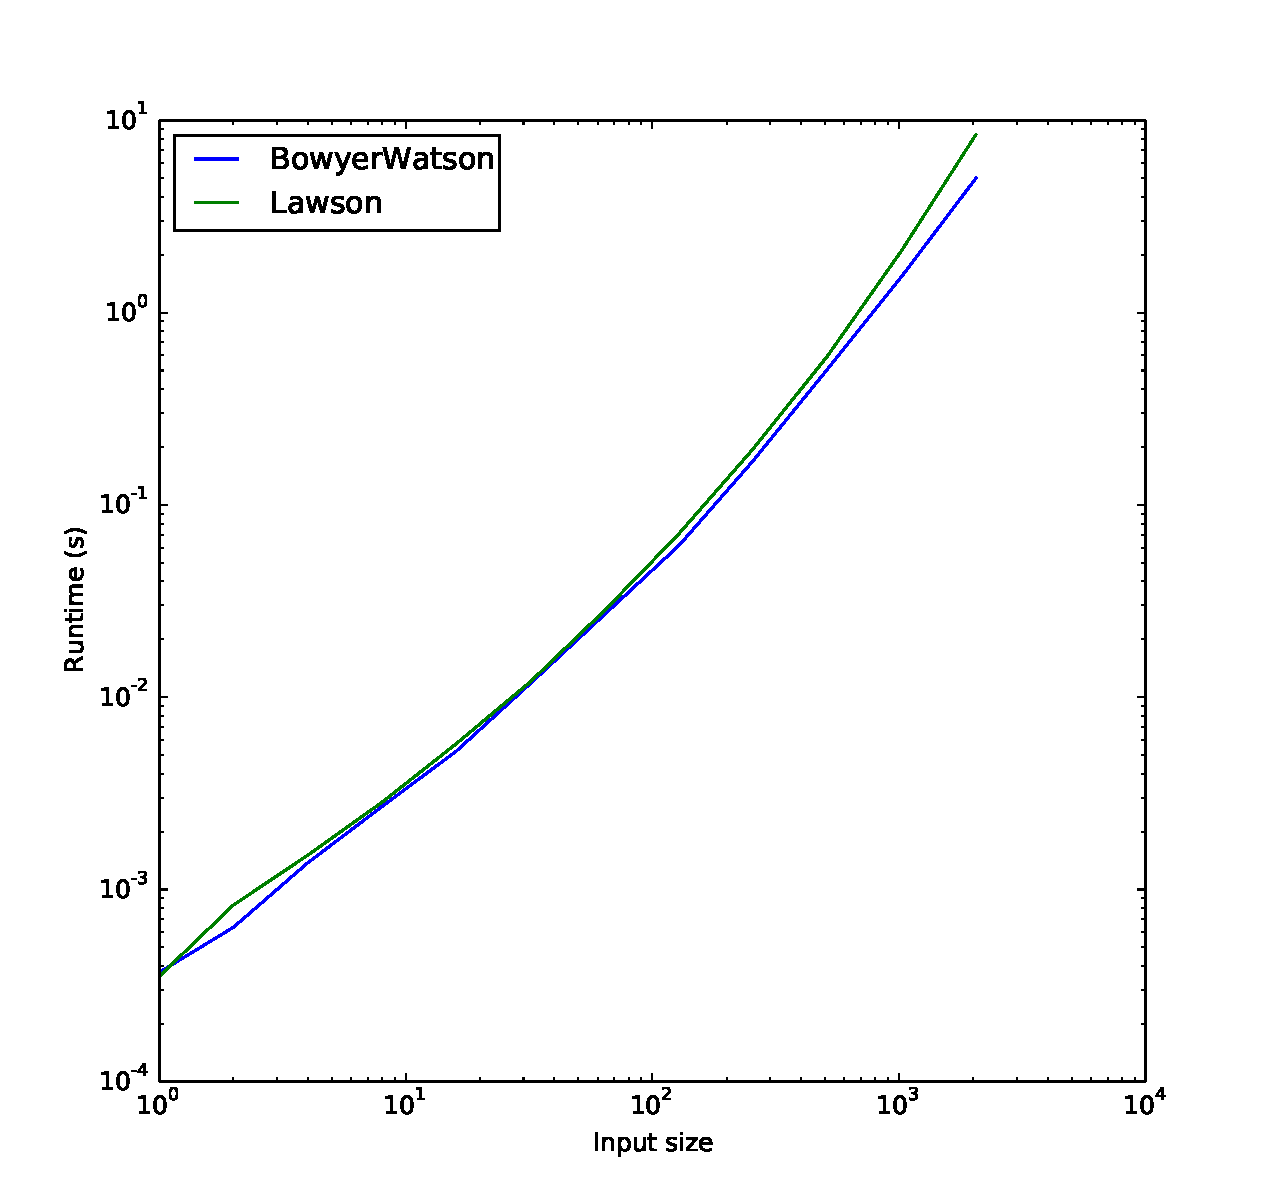
\includegraphics[width=\columnwidth]{../images/runtime_segments.pdf}
    \caption{Runtime for triangulation algorithms when input is constrained by a PSLG}
    \label{fig:triangulation-pslg-runtime}
\end{figure}

\subsection{Ruppert's refinement algorithm}
\label{sub:results:ruppert}

Ruppert's algorithm has been ran on the boundary of a car.
Two parameters of the algorithm were varies.
The maximum area of each triangle was restricted to values ranging from $50$ to $300$.
The minimum angle in each triangle was restricted to values ranging from $10\degr$ to $300\degr$.
Unfortunately, the algorithm didn't converge for each setting, so the algorithms were cut off when they ran for more than $10$ seconds.
An example of a triangulation obtained by running Rupperts algorithm can be found in Figure \ref{fig:result_Car20}.

In Figure \ref{fig:ruppert-runtime} we see the runtime for different minimum angles and in Figure \ref{fig:ruppert-runtime2} we see the runtime for different maximum areas.
From the graph we notice that the algorithm seems to converge fastest when we limit the smallest angle to about $23\degr$.
When the angles are either big or small, the algorithm converges at a much slower rate.
Making the maximum area bigger, seems to make the runtime slightly slower.
Surprisingly, setups in which the maximum area is divisible by 100 seem to converge faster than other setups.

\begin{figure}[ht]
    \centering
    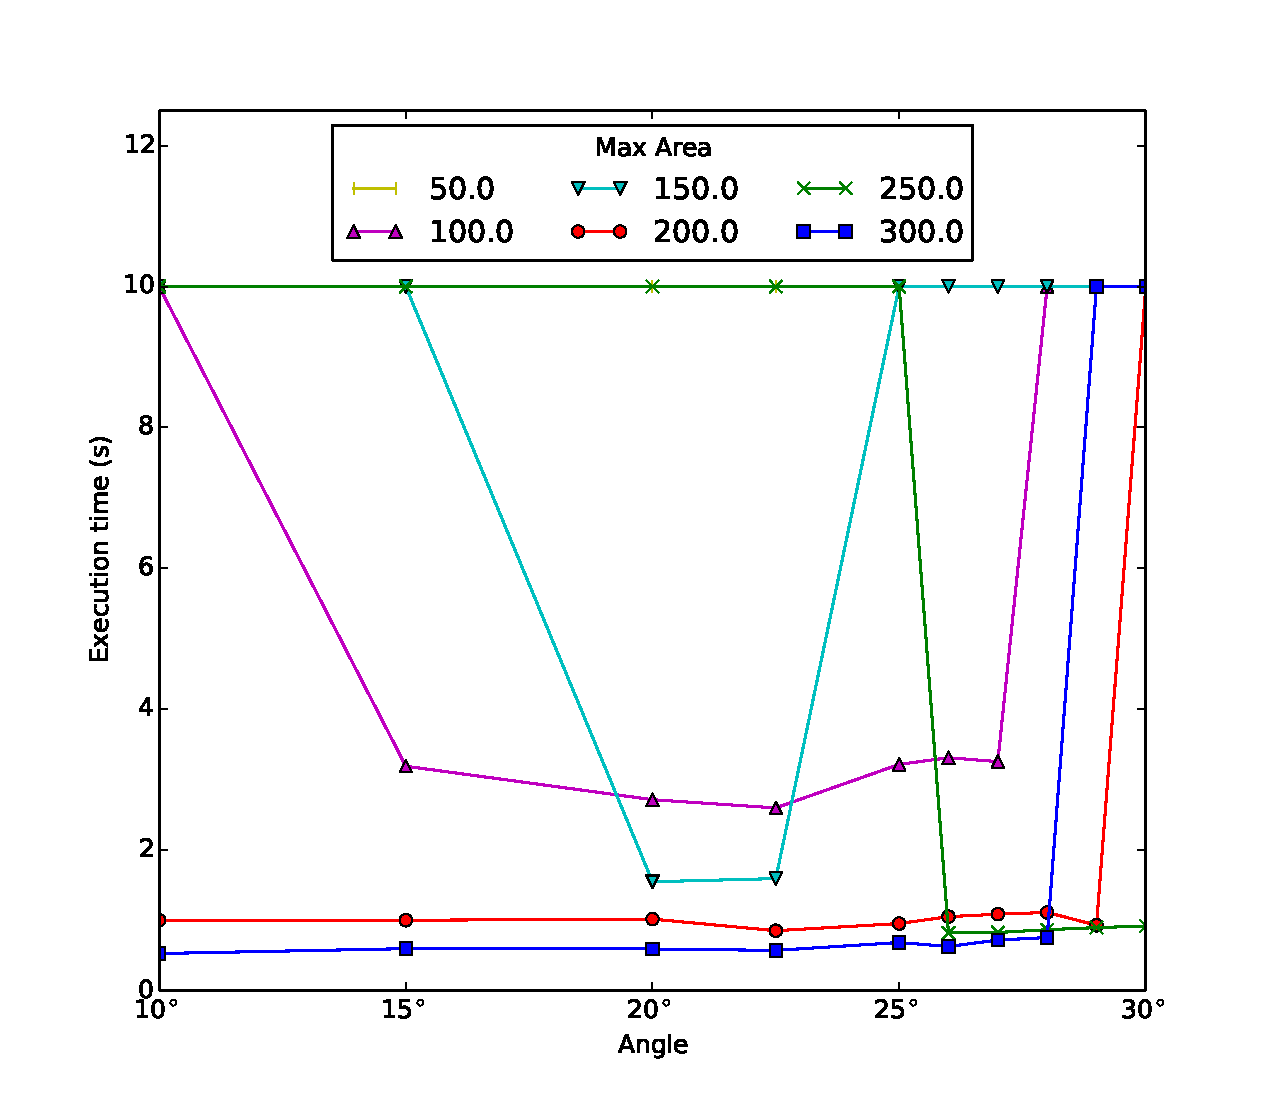
\includegraphics[width=\columnwidth]{../images/ruppert.pdf}
    \caption{Runtime of Ruppert's algorithm for different angles}
    \label{fig:ruppert-runtime}
\end{figure}

\begin{figure}[ht]
    \centering
    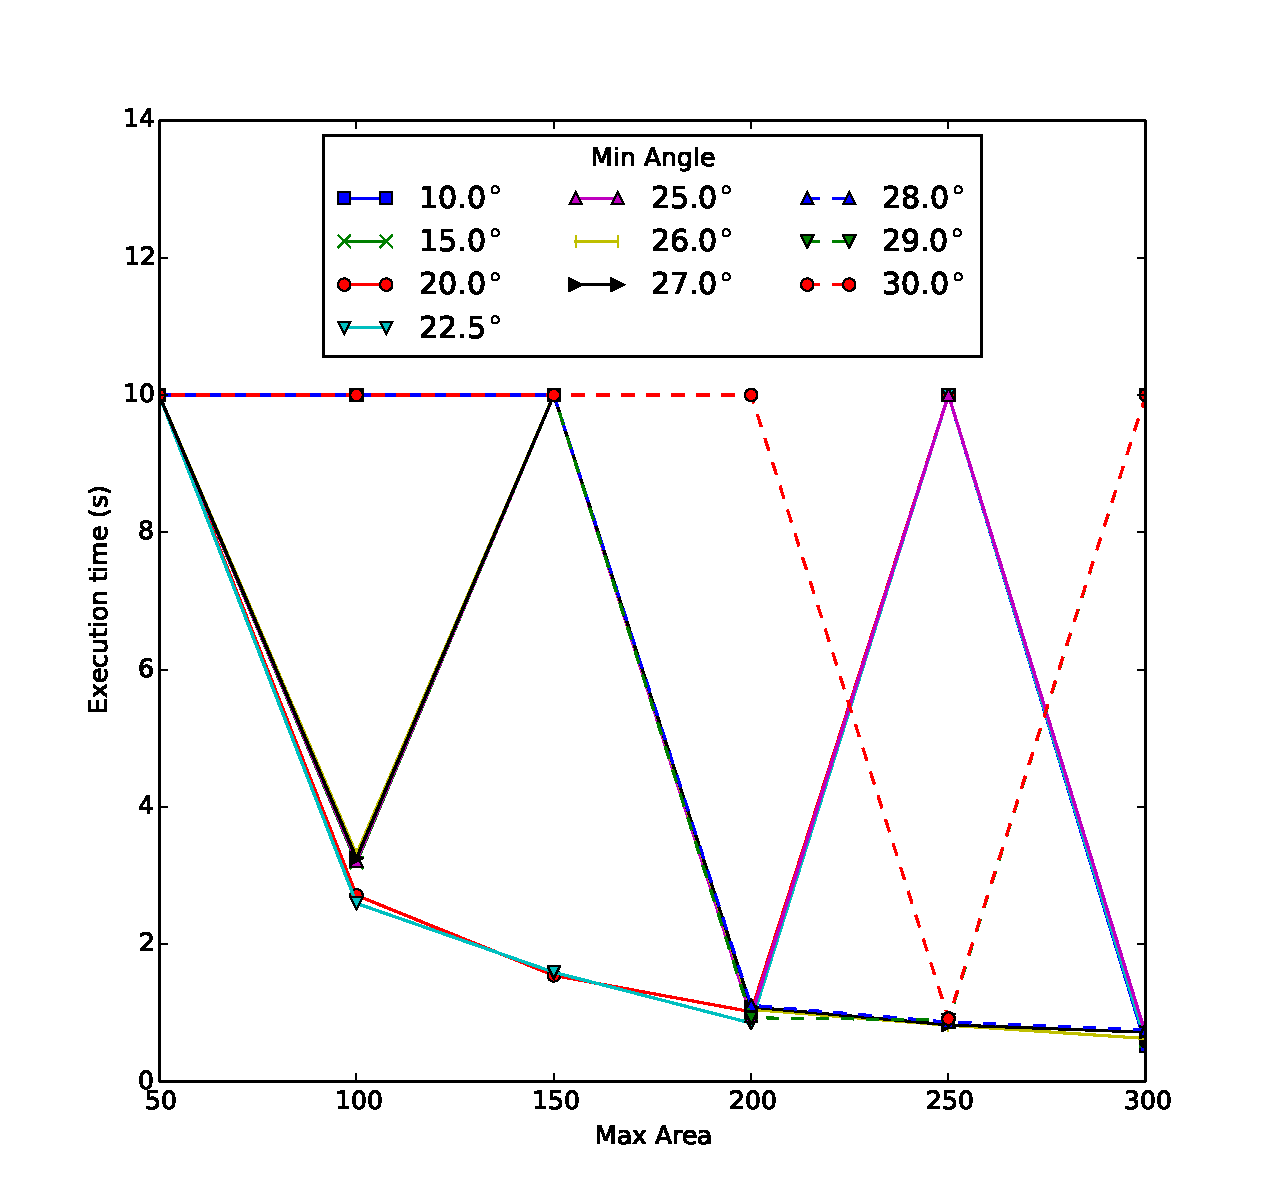
\includegraphics[width=\columnwidth]{../images/ruppert2.pdf}
    \caption{Runtime of Ruppert's algorithm for different max areas}
    \label{fig:ruppert-runtime2}
\end{figure}

\begin{figure}
    \centering
    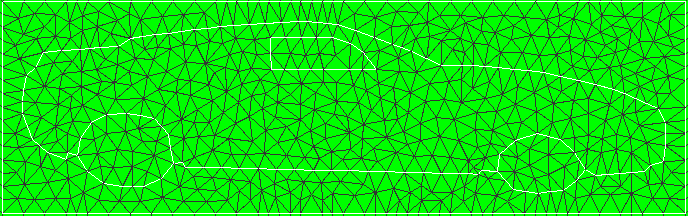
\includegraphics[width=\columnwidth]{../images/Car_Ruppert20.png}
    \caption{Triangulation generated using Ruppert's refinement algorithm for a car. The white lines are PSLG boundary elements.
    The criterea were set to a minimum angle of 20$\degr$ and a maximum area of 200.}
    \label{fig:result_Car20}
\end{figure}

\begin{figure}
    \centering
    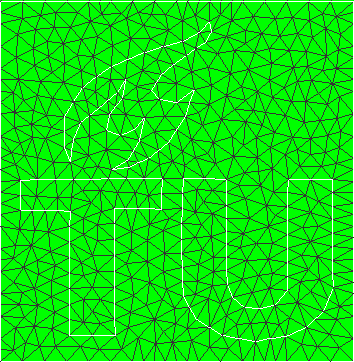
\includegraphics[width=\columnwidth]{../images/TU_Ruppert20.png}
    \caption{Triangulation generated using Ruppert's refinement algorithm for the TU Delft logo. The white lines are PSLG boundary elements.
    The criterea were set to a minimum angle of 20$\degr$ and a maximum area of 200.}
    \label{fig:result_TU20}
\end{figure}

